\chapter{Results}\label{chapter:results}

%\section{The issue with inconsistent energy readings} \label{sec:results_the_issue_with_inconsistent_energy_readings}

In this section we will report the results of the experiments conducted to evaluate the framework and its components. The results will be presented in a structured manner, focusing on the performance of the program generator, the orchestrator, the model training, and the extension tool. Each section will provide insights into the effectiveness of the framework in measuring and predicting energy consumption in Java programs.

Our hardware infrastructure is composed of two systems, one high-performance workstation used for data generation and collection, and a lower-spec machine used for testing the extension tool. The high-performance workstation is equipped with an AMD Ryzen Threadripper 3960X CPU, 94 GiB of RAM, and an NVIDIA GeForce RTX 3090 Ti GPU, while the lower-spec machine has an AMD Ryzen 5 3600 CPU, 16 GiB of RAM, and an NVIDIA GeForce RTX 3060 Ti GPU. The details of the hardware specifications can be found in Table~\ref{tab:hardware_specs}.

\begin{table}[htbp]
  \small
  \centering
  \caption{Hardware Infrastructure Specifications}
  \label{tab:hardware_specs}
  \begin{tabularx}{\textwidth}{l X}
    \toprule
    \textbf{Component} & \textbf{Specification} \\
    \midrule
    \multicolumn{2}{l}{\textbf{System 1 — Data Generation and Collection (High-Performance Workstation)}} \\
    \cmidrule(r){1-2}
    OS & Ubuntu 24.04.2 LTS (x86\_64) \\
    CPU                 & AMD Ryzen Threadripper 3960X (24 cores / 48 threads). 2.2 GHz, up to 5.05 GHz \\
    RAM                 & 94 GiB \\
    GPU                 & NVIDIA GeForce RTX 3090 Ti (GA102) with 24 GiB VRAM \\
    \midrule
    \multicolumn{2}{l}{\textbf{System 2 — Machine for Testing (Lower-Spec)}} \\
    \cmidrule(r){1-2}
    OS                  & Ubuntu 24.04.2 LTS (x86\_64) \\
    CPU                 & AMD Ryzen 5 3600 (6 cores / 12 threads). 3.6 GHz, up to 4.2 GHz \\
    RAM                 & 16 GiB \\
    GPU                 & NVIDIA GeForce RTX 3060 Ti with 8 GiB VRAM \\
    \bottomrule
  \end{tabularx}
\end{table}


The more powerful system, System 1, as described in Table~\ref{tab:hardware_specs}, was used for program generation and data collection, as it was configured to work with SLURM (Simple Linux Utility for Resource Management). SLURM is a highly scalable, open-source job scheduler used to efficiently manage compute resources on shared systems. It allows tasks to be queued and scheduled based on resource availability and job priority, helping to organize workloads across users without manual intervention. The model training did not use SLURM, as it did not require significant computation capabilities.

At the beginning of the experiment, some tools (described in Section \ref{sec:background_energy}) were tested to observe their behavior, understand how to use them, and determine which one best suited the needs of the project.

During the initial testing, Experiment Runner~\cite{S2_Group_Experiment_Runner}, a Python framework designed to facilitate experiment measurements was our tool of choice. The framework included an initial test template that used PowerJoular to measure energy of programs. While using the template and testing the framework some bugs and unexpected results were found, some of which were due to misuse of the framework.
Due to these issues, a tailor-suited Java orchestrator was developed. Although it performed the same core function as Experiment Runner (measuring energy consumption), it was more straightforward, focusing exclusively on energy measurement rather than providing a general-purpose solution.

However, some discrepancies were observed between the energy values measured by the Java and Python frameworks. This was unexpected, as both used the same energy measurement tool (PowerJoular) and measured the same program in the same way. Still, the Python framework consistently reported lower energy values than the Java version.
To investigate which tool was causing the inconsistency, \st{two} \wo{three} more orchestrators were implemented, including a simplified Python version. In total, four orchestrators were developed: Java, Python, C, and Bash. All four performed the same process, calling PowerJoular to measure the energy usage of a Java program.
This setup represents an early iteration of the approach later detailed in Section~\ref{sec:work_stage2_orchestrator}, which utilized signal-based control to ensure that the measurement tool only ran during the exact computation period being measured.

Figure~\ref{fig:4_orchs_comparison} presents the used CPU power observed by the four orchestrators while running 
 100 times a Fibonacci recursive program written in Java. They are ordered by the less energy to the highest energy. \st{And it shows the energy reads for the four different orchestrators used.} The labels contain the average energy values and its standard deviation.

\begin{figure}[htbp]
  \centering
  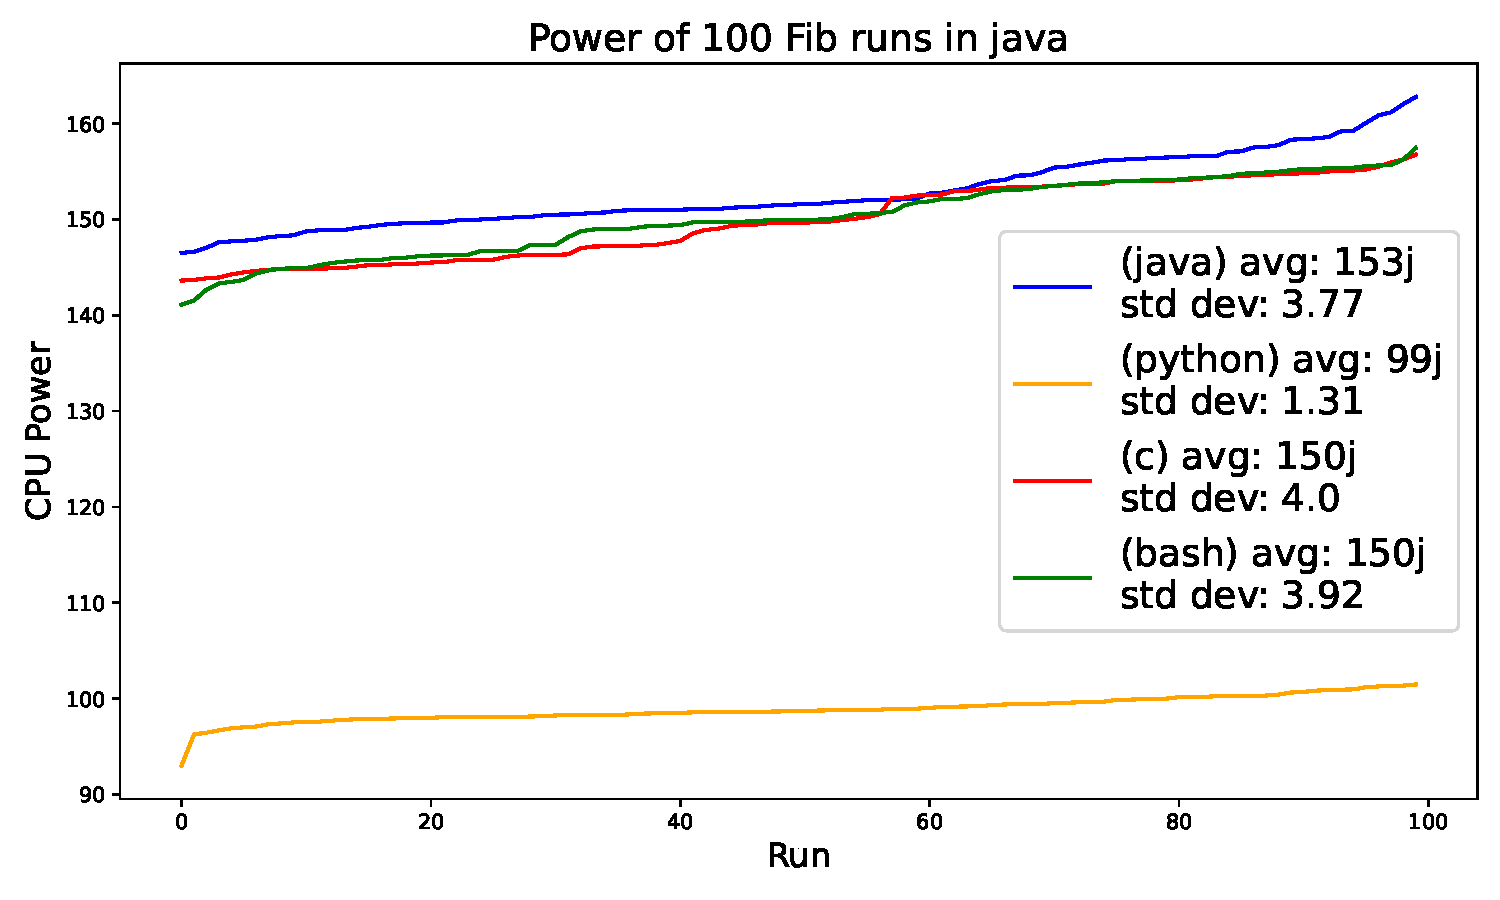
\includegraphics[width = .8 \textwidth]{figures/4_orchs_comparison.pdf}
  \caption{Orchestrators Comparison}
  \label{fig:4_orchs_comparison}
\end{figure}

It is noticeable that the Python orchestrator read energy values lower than the other orchestrators. Further analysis of the orchestrators revealed a notable difference in behavior. When the Python orchestrator was running, both the parent and child processes consumed CPU resources. In contrast, the other orchestrators (Java, C, and Bash) showed CPU usage only in the child process. This disparity may explain why PowerJoular reported lower energy consumption for the Python orchestrator. Since the CPU load was shared between the parent and child processes, PowerJoular, which measures energy only for the child process (in this example, the target Fibonacci program), captured less total energy usage.
Since the experiment runner included an example demonstrating how to use the framework with PowerJoular, the authors were made aware of this potential conflict when launching PowerJoular from Python, {\color{blue}having been warned of this potential conflict via email}.


\section{Models Metrics} \label{sec:models_metrics}

To instantiate the tool, models were trained on methods from the Java collections framework, specifically focusing on the \texttt{List} and \texttt{Map} interfaces. Data for these methods was generated, collected, and used to train the models. With the models in place, it is now possible to evaluate their performance using metrics such as R² and Mean Squared Error (MSE), based on the features extracted during data collection.

%\begin{figure}[htbp]
%  \centering
%  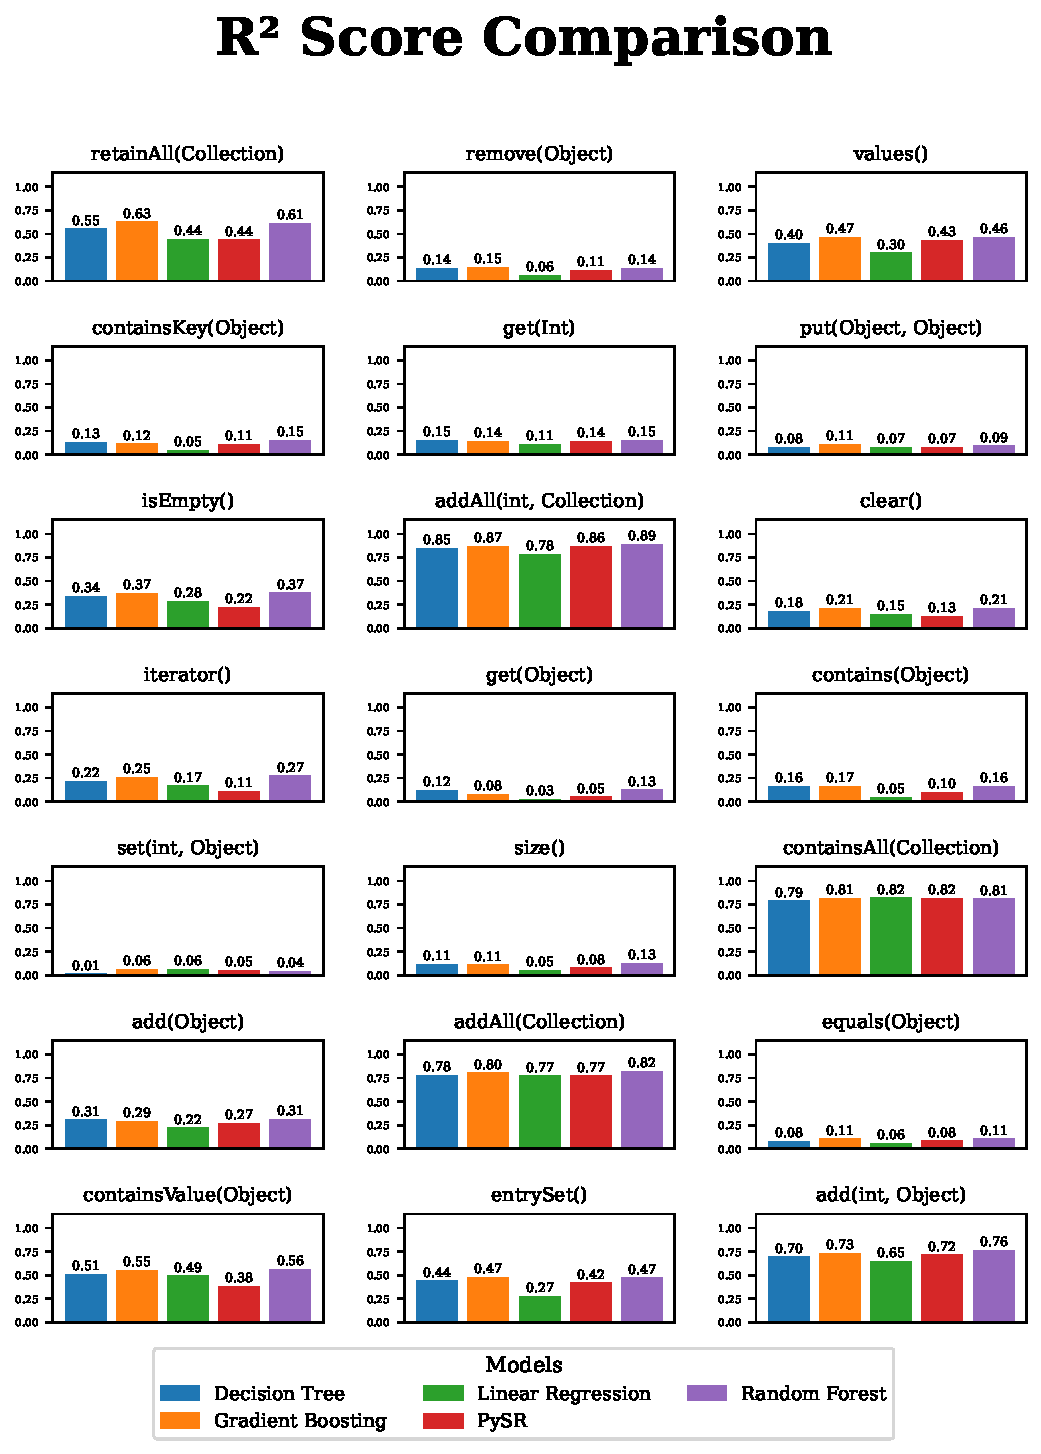
\includegraphics[width=0.85\textwidth]{figures/r2_comparison.pdf}
%  \caption{R² Comparison (\textit{Higher is better})}
%  \label{fig:r2_comparison}
%\end{figure}

Figure~\ref{fig:r2_comparison} presents the R² of all the methods that were analyzed from the \texttt{List} and \texttt{Map} interfaces. A score of 1 would mean that the model can get 100\% of the prediction right\. However, most of the time, it is not feasible to achieve a score of 1. In fact, most values are really low (bellow 0.5), which means that the model cannot predict the energy very well for some methods. The best models were for the method \texttt{addAll()} and \texttt{containsAll()} of the \texttt{List} collection, which got an R² of around 0.8 for most models.

\begin{figure}[htbp]
  \centering
  \makebox[\textwidth][c]{%
    \hspace{5mm}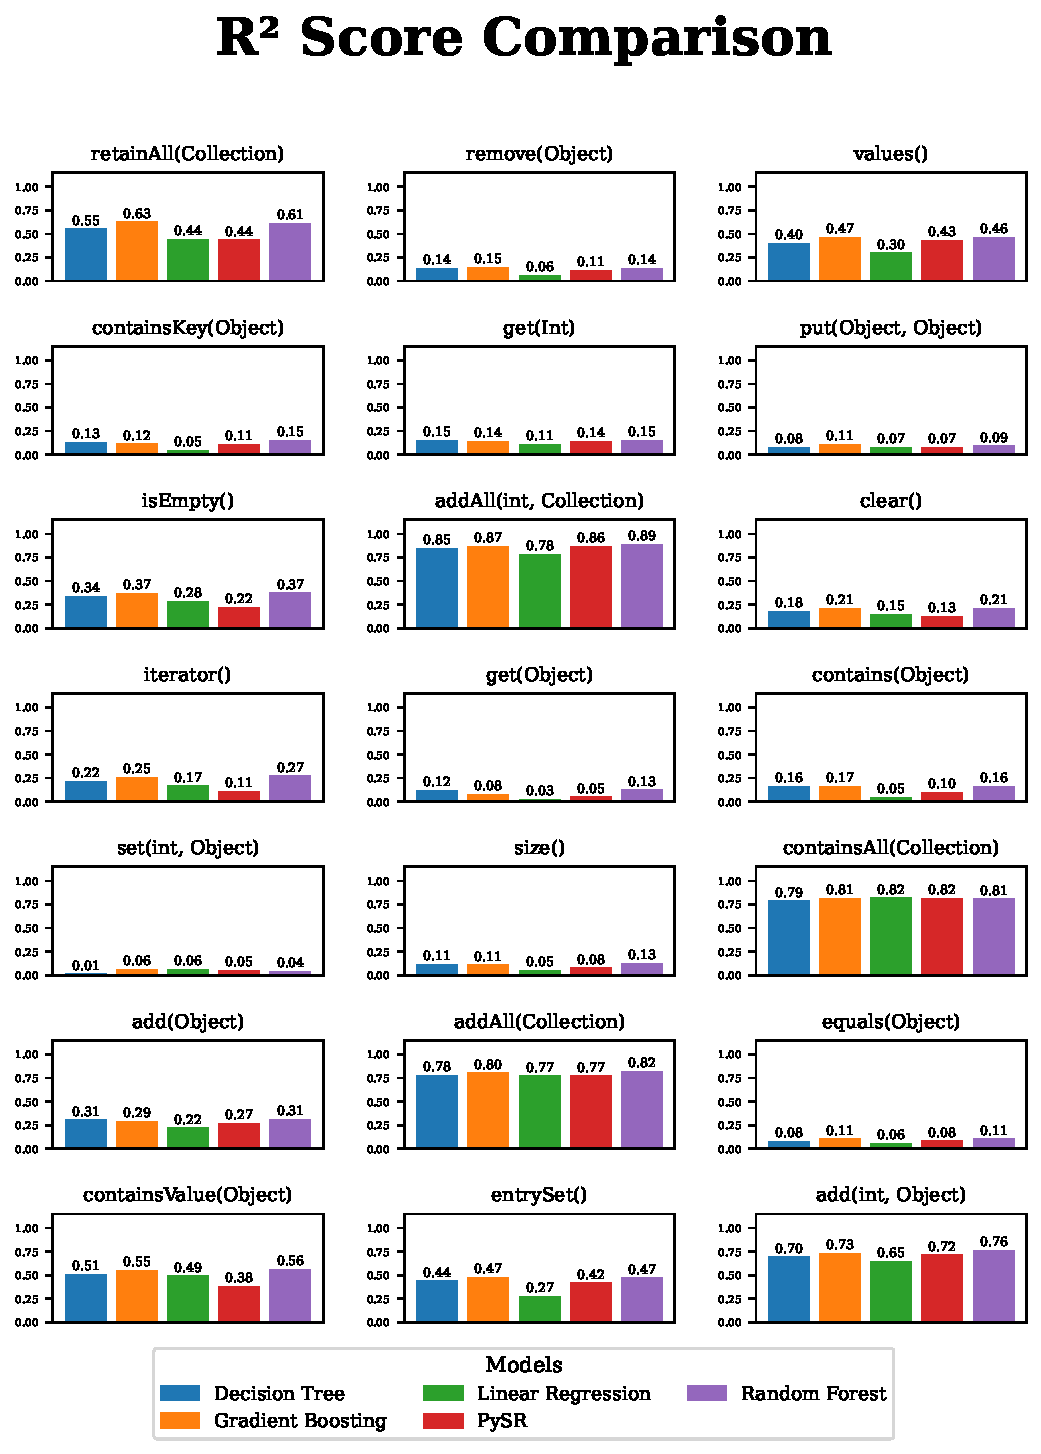
\includegraphics{figures/r2_comparison.pdf}
  }
  \caption{R² Comparison (\textit{Higher is better})}
  \label{fig:r2_comparison}
\end{figure}

These three methods with the highest accuracy were the ones that generated bigger energy outputs, because the methods were computationally more intenstive than the others. This made it so that bigger inputs would result in bigger energy outputs, and make the models more easily find a pattern to predict the energy. As for the other models, since a bigger input would not mean a bigger energy output, the model, might have some difficulties predicting the energy. This does not mean that a lower R² will completely make the model unusable for some methods, as their MSE, that can be seen in the Figure~\ref{fig:mse_comparison} is not high, meaning that even when failing to predict the energy of the method, the failed prediction will not be far away as one might expect. For example, if a model has an MSE of $1 \times 10^{-10}$ and predicts the energy usage to be $1~\mathrm{J}$, then even if the prediction is not exact, the true value is likely within $\pm \sqrt{1 \times 10^{-10}} = \pm 1 \times 10^{-5}~\mathrm{J}$ of the prediction, indicating accurate performance despite a potentially low R². 

\begin{figure}[htbp]
  \centering
  \makebox[\textwidth][c]{%
    \hspace{5mm}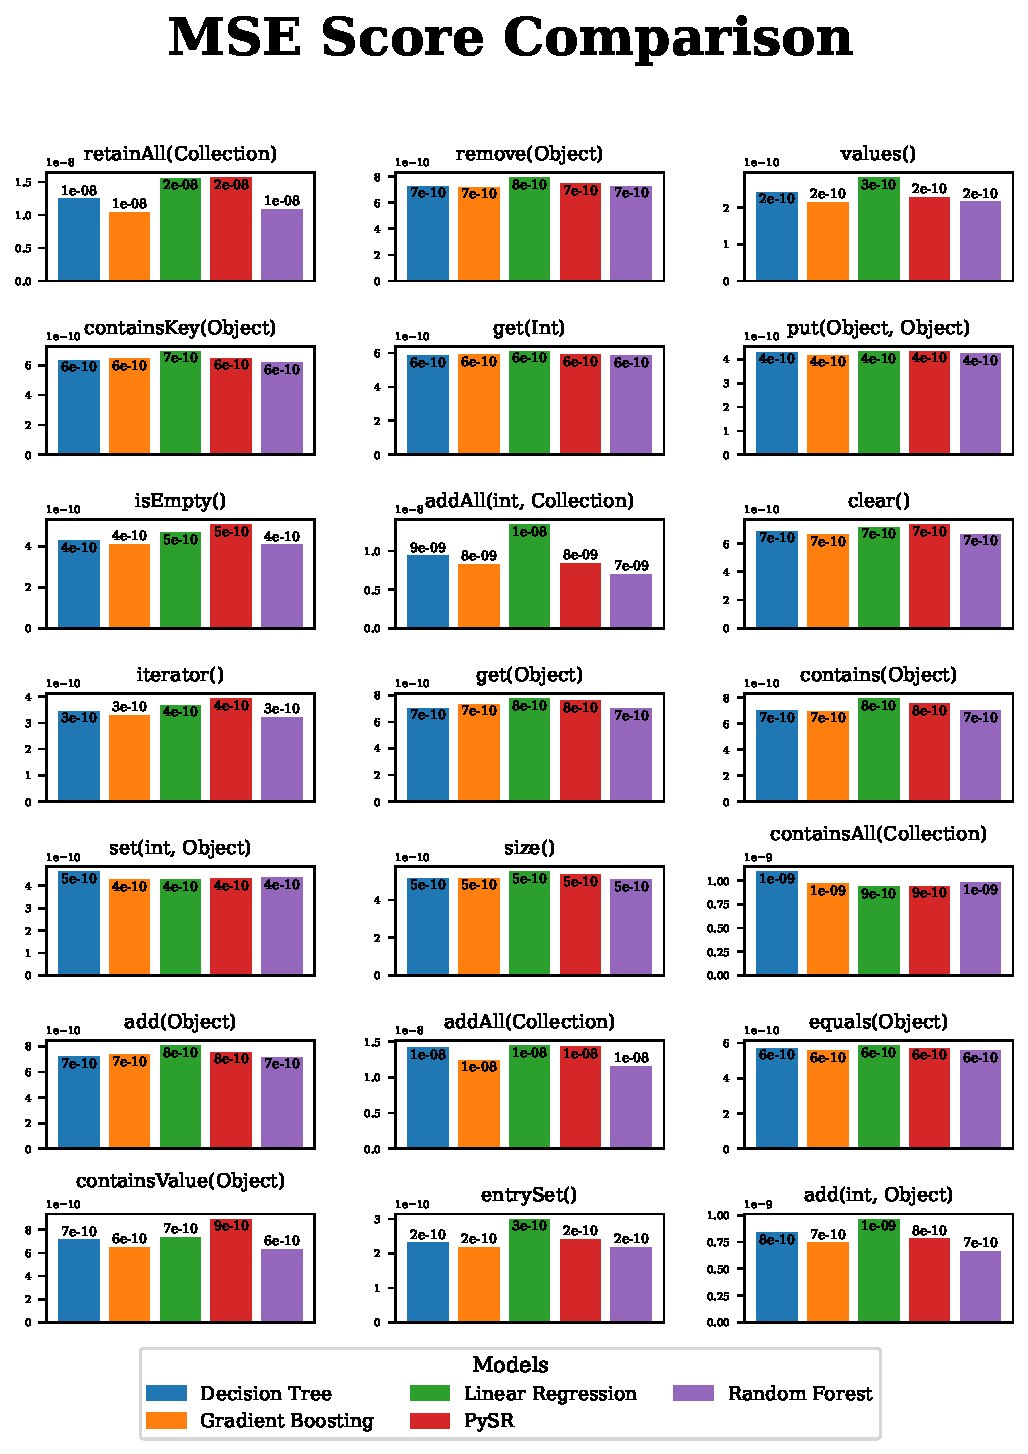
\includegraphics{figures/mse_comparison.pdf}
  }
  \caption{MSE Comparison (\textit{Lower is better})}
  \label{fig:mse_comparison}
\end{figure}

Another factor that may contribute to low R² scores is the behavior of the energy measurement tool when applied to certain methods. For instance, some methods, such as \texttt{size()}, do not require more computational effort as the collection size increases. Whether the collection has one element or one million, the method executes in roughly the same amount of time. Consequently, the energy consumption remains nearly constant, regardless of the input size. Since these methods complete \st{very} quickly and consume \st{very} little energy, even minimal measurement noise can significantly affect the recorded values. Figure~\ref{fig:size_energy} illustrates this effect: although an increase in energy with input size is typically expected, the recorded energy values for \texttt{List.size()} remain considerably flat. While this example isolates a single feature, and other features also influence energy consumption, input size is often the most significant. This observation suggests that for low-energy, low-variance methods, measurement noise can impact the signal, making accurate energy prediction particularly challenging.

\begin{figure}[htbp]
  \centering
  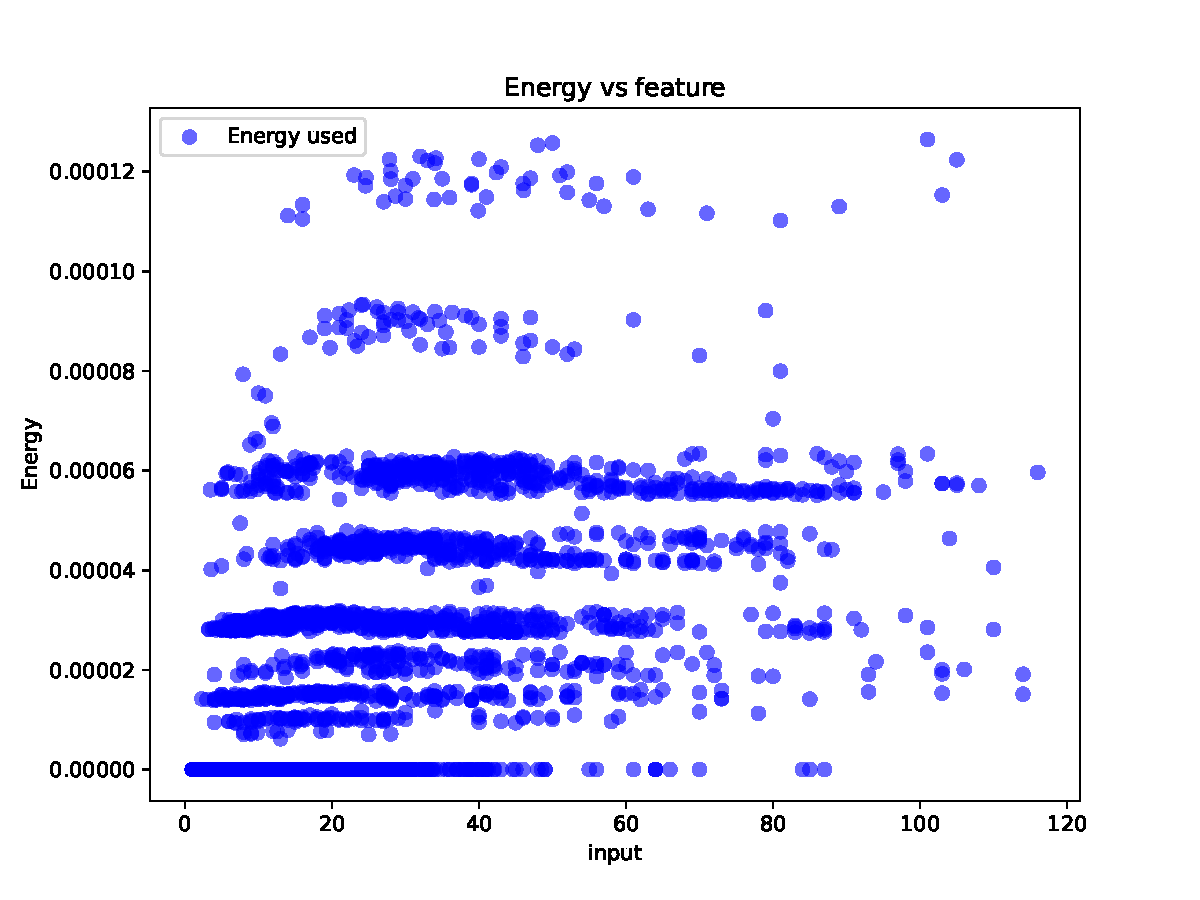
\includegraphics[width = .8 \textwidth]{figures/size_energy.pdf}
  \caption{Energy for the \texttt{List.size()} method with different list sizes.}
  \label{fig:size_energy}
\end{figure}


Nonetheless, the lower R² scores should be addressed, and what can be done to improve the results of these models is to have the program generator create higher inputs, so the energy profiles also have outputs with higher energy, making the energy predictions more accurate. Then, since most of the predictions depend on the input, it means the other features do not have such higher impact, so it is also important to pick better features and remove others that might not be interesting. {\color{blue}It is possible to improve a complex method that relies on a simpler method by incorporating the features or predictions of the simpler method, which can help improve the accuracy of the model for the complex method. In particular, accessing the energy profiles of simpler methods may refine the R² score of the complex method, as part of its behavior can be decomposed into more predictable components.}



In general, most of the models present similar scores, however we used PySR in the instantiation. The biggest advantage over the other models is that it can represent the predictions in expressions which can help the users to try to understand why the code is using more energy. It has a nice feature of allowing to balance complexity and accuracy. And can easily be used in another code language as it is represented as a mathematical expression.
The fact that most models present similar results, ranging from advanced models like Random Forest and Gradient Boosting to simple models like Linear Regression, suggests that features used in the model likely do not capture highly nonlinear or complex relations. This indicates that energy consumption behavior in analyzed approaches can be reliably captured by simple relations. As a result, the set of features cannot offer the richness or variability needed for distinguishing more subtle energy behavior. This does not mean that the learning problem is simple, rather, it indicates that the available features may fail to express potential nonlinear patterns of energy consumption. Although the strategy should be enough for most cases, to improve prediction performance and enable more effective use of expressive models, future work should incorporate features capable of highlight the complexity of predicting energy usage.



\section{Predicted vs. Measured Energy} \label{sec:predicted_vs_measured_energy}

Leveraging the developed models and the extenstion, we can present the results and evaluate how accurately the tool estimates energy consumption compared to real measurements obtained using PowerJoular. Since the energy profiles were generated on a specific hardware setup (see Table~\ref{tab:hardware_specs}), the resulting models are adjusted to that particular system. If the tool were run on a different machine, the absolute energy values would likely differ due to variations in hardware characteristics. However, the relative differences in energy consumption between operations are expected to remain consistent. For instance, if \texttt{TreeMap} consumes more energy than \texttt{HashMap} on one system, the same trend will likely hold on another system, even if the exact energy values vary.

\begin{listing}[H]
\noindent\rule{\linewidth}{0.4pt}
\begin{minted}[linenos, fontsize=\small, frame=none, bgcolor=white,breaklines=true,breakanywhere=true]{Java}
    ArrayList<Integer> l = new ArrayList<>();
    ArrayList<Integer> l2 = new ArrayList<>();
    l.addAll(l2);
\end{minted}
\noindent\rule{\linewidth}{0.4pt}
\caption{Code example}            
\label{lst:code_example}
\end{listing}

To test the extension tool accuracy, the energy measurement needs to be run in the same machine were the data was collected. It is also important to take into account that the measured energies from these experiments were not processed exactly like the orchestrator, as the orchestrator processer has a more general approach that can introduce overhead in some cases. {\color{blue}So the experiments performed, when possible, were only measuring the exact targeted method. For example, to measure the method \texttt{foo(type)} the orchestrator would need to create an array of parameters and loop through it during 1 second or until the end of the array size. However, during these experiments, if a single invocation of the method was sufficient for PowerJoular to capture its energy consumption, then only that single call was performed. This minimizes overhead and more accurately reflects real-world usage scenarios}.

For this a simple program was developed, Listing~\ref{lst:code_example}, more like simple Java instructions, of just creating two lists (both with size 1000) and using the method \texttt{addAll(Object)} and checking if the prediction matches the actual measurement.

\begin{table}[htbp]
  \centering
  \label{tab:energy_comparison}
  \footnotesize
  \begin{tabular}{>{\raggedright\arraybackslash}p{4cm}ccc}
    \toprule
    Method & Actual Energy Range (J) & Predicted Energy (J) & Prediction Error (\%) \\
    \midrule
    \texttt{addAll(Object)} & 4.9e-4 -- 5.1e-4 & 5.51e-4 & 10.2 \\
    \midrule
    \texttt{addAll(Object)} + \texttt{size()} + \texttt{equals(Object)} & 5.0e-4 -- 5.2e-4 & 6.49e-4 & 27 \\
    \midrule
    \texttt{Map.put(Object, Object)} + \texttt{loop(1000)} & 0.0027 -- 0.0030 & 0.033 &  1058 \\
    \bottomrule
  \end{tabular}
  \vspace{0.5em}
  \caption{Comparison of actual and predicted energy consumption for different methods}
  %\footnotesize{The actual energy ranges were obtained by running the program 10 times.}
\end{table}


%\begin{table}[htbp]
%  \centering
%  \footnotesize
%  \makebox[\textwidth][c]{%
%    \begin{tabular}{@{}p{5cm}@{\hspace{2.5em}}c@{\hspace{0.5em}}ccc@{}}
%      \toprule
%      Method & Actual Energy Range (J) & Predicted Energy (J) & Input Value (\%) & Prediction Error (\%) \\
%      \toprule
%      \texttt{BinaryTrees.createTree(int)} & 3.75e-4 -- 4.60e-4 & -0.083 & 10 & 19980 \\
%      \midrule
%      \texttt{BinaryTrees.createTree(int)} & 11.78 -- 12.63 & 10.26 & 23 & 15.9 \\
%      \midrule
%      \texttt{BinaryTrees.createTree(int)} & 77.29 -- 80.63 & 79.90 & 26 & 1.2 \\
%      \midrule
%      \texttt{BinaryTrees.checkTree(TreeNode)} & 1.64e-4 -- 1.75e-4 & 1.88e-4 & 10 & 10.9 \\
%      \midrule
%      \texttt{BinaryTrees.checkTree(TreeNode)} & 1.37 -- 1.56 & 2.19e-3 & 23 & 99.85 \\
%      \midrule
%      \texttt{BinaryTrees.checkTree(TreeNode)} & 11.72 -- 13.29 & 3.15e-3 & 26 & 99.97 \\
%      \midrule
%      \texttt{BinaryTrees.trees(int)} & 0.041 -- 0.045 & -3.42 & 10 & 127 \\
%      \midrule
%      \texttt{BinaryTrees.trees(int)} & 713 -- 800 & 517.89 & 23 & 31.59 \\
%      \midrule
%      \texttt{BinaryTrees.trees(int)} & 6260 -- 7111 & 2429 & 26 & 63.66 \\
%      \midrule
%      \texttt{BinaryTrees.checkTree(TreeNode) + createTree(int) + trees(int)} & 4.59e-2 -- 4.77e-2 & -3.49 & 10 & 7578 \\
%      \midrule
%      \texttt{BinaryTrees.checkTree(TreeNode) + createTree(int) + trees(int)} & 796 -- 806 & 528.15 & 23 & 34.08 \\
%      \midrule
%      \texttt{BinaryTrees.checkTree(TreeNode) + createTree(int) + trees(int)} & 7062 -- 7350 & 2509 & 26 & 65.18 \\
%      \bottomrule
%    \end{tabular}%
%  }
%  \caption{Comparison of actual and predicted energy consumption for BinaryTrees program}
%  \label{tab:energy_comparison_bin_trees}
%\end{table}


The actual value measured by PowerJoular is in the range of 4.9e-4 to 5.1e-4J while the prediction is 5.51e-4J. This shows that the prediction (about 10.2\% prediction error) was good for this method in particular.
When trying to add two more operations (\texttt{size()} and \texttt{equals(Object)}) the measurement is in the range of 5.0e-4 to 5.2e-4J and the prediction is 6.49e-4J, about (about 27\% prediction error). Usually, the method \texttt{addAll(Object)} is one of the methods that has the best accuracy of around 80\%. Composing \texttt{addAll(Object)} with the other methods (\texttt{size()} and \texttt{equals(Object)}) that presented a low R² creates a more complex behavior and, as expected, increases the prediction error. Although the prediction is not as accurate as the previous one, it still provides a reasonable estimate of the energy consumption.

However, if we use the program presented in Listing~\ref{lst:Java_program_to_count_word_frequencies_in_a_string}, which involves a Map and a loop, the prediction accuracy drops significantly. The actual energy measured is in the range of 0.0027J to 0.0030J, while the prediction is 0.033J, resulting in a prediction error of about 1058\%. This discrepancy highlights the limitations of the model when applied to more complex operations involving Maps and loops.

The models trained have a low accuracy for Map methods. The prediction error is very high, which means that the model is not able to predict the energy consumption of these methods accurately. This is likely due to the fact that the models were trained on a limited set of data and do not generalize well to more complex operations.

This issue also highlights a limitation of our instantation: by composing with methods that have low R² scores, the prediction accuracy is significantly affected. The models trained on methods with low R² scores struggle to accurately predict energy consumption for more complex operations, leading to high prediction errors, which leads to an error accumlation problem. Potential solutions could involve introducing a correction factor or calibration step based on empirical error measurements, adjusting the final predicted value to better reflect observed trends.

{\color{blue}The results demonstrate that the extension tool is capable of providing useful estimations, especially in terms of relative trends between methods and input sizes. Proving it is capable of helping software developers on being more aware of the energy consumption of their codes. It shows potential in prediction, especially, for methods that are more impacted by the input. However, it is noteworthy that not all methods had the same high prediction accuracy as \texttt{addAll(Object)}, and combining multiple methods or increasing program complexity tends to amplify prediction errors.
These limitations highlight the importance of carefully selecting input sizes and operations for meaningful energy analysis, and they suggest that the tool is best suited for relative comparisons rather than precise energy estimation.}

\wo{eu não gosto muito do tom aqui, parece que estás a dizer que o tool tem mais problemas do que solução. Acho que precisamos falar das limitações, claro, mas precisamos dar ênfase ao que fazemos bem. Seria bom reescrever isto para que o tom seja mais positivo, e que se foque mais no que conseguimos fazer bem, e menos no que não conseguimos fazer. Eu percebi que em todos os casos que tu mostrou os erros foram que superestimamos o consumo energético. Consegues apontar algo nessa direção? Por qual motivos os modelos que treinamos acham que o código vai usar muito mais energia do que realmente usa? E o que podemos fazer para melhorar isso?}


\section{Evaluating Java Benchmark Programs} \label{sec:evaluating_java_benchmark_programs}

Our previous experiments were designed to evaluate simple methods, but we also used test cases considered more realistic, to further evaluate the framework’s ability to analyze and collect energy models for various custom programs. The programs were selected from the Computer Language Benchmarks Game~\cite{benchmarksGameJava}, which provides algorithmic benchmarks designed to test language performance on tasks that are representative of certain real-world computational workloads. The chosen programs were \texttt{BinaryTrees} (Java naot \#3) \texttt{fannkuch-redux} (Java), \texttt{n-body} (Java naot \#4), and \texttt{spectral-norm} (Java). These benchmarks were specifically selected because they are purely CPU and memory bound, with minimal variability, no reliance on disk I/O or multithreading, and no usage of external libraries. This makes them more predictable and reliable for energy consumption measurements.


{\color{blue}Starting with the program \texttt{BinaryTrees}, which implements a classic performance benchmark that builds, traverses, and destroys many binary trees to stress the memory allocation and garbage collection systems. It is composed of three main methods, some of which perform computationally intensive tasks, described as follows:}

\begin{itemize}
  \item \texttt{createTree:} Recursively builds a binary tree of the given depth. At each level, creates a node with two children (left and right), until depth equals zero. The result is a complete binary tree with \(2^{\text{depth}} - 1\) nodes.
 
  \item \texttt{checkTree:} Recursively traverses the tree and counts the number of nodes. For leaf nodes, it returns \texttt{1}. For internal nodes, it returns the sum of the recursive calls on the left and right subtrees plus one: $1 + \text{check(left)} + \text{check(right)}$.
  
  \item \texttt{trees:} Performs the core part of the benchmark by creating and checking many binary trees of varying depths and keeping one long-lived tree in memory to simulate memory pressure.
\end{itemize}

{\color{blue}The \texttt{fannkuch-redux} program also presents a computationally intensive task. It generates all permutations of the sequence \([0, 1, \ldots, n-1]\) and, for each permutation, performs a "flip" operation until the first element is zero. A flip consists of reversing the order of the first \(k + 1\) elements, where \(k\) is the first element of the permutation. For each permutation, it tracks the number of flips needed (called the flip count) and maintains the maximum flip count across all permutations. Additionally, it calculates a checksum by adding or subtracting the flip count based on the parity of the permutation index. The function returns the maximum number of flips needed for any permutation.

The \texttt{spectralnorm} program computes an approximation of the spectral norm (largest singular value) of a specific, implicitly defined matrix. It uses the power method, an algorithm that repeatedly multiplies a vector by the matrix to estimate how strongly the matrix can amplify a vector. The matrix \(A\) is not stored explicitly, instead, each element is computed on demand using the formula \(A_{i,j} = \frac{1}{\frac{(i + j)(i + j + 1)}{2} + i + 1}\). The program initializes a unit vector and performs 20 steps of power iteration by repeatedly multiplying with \(A\) and its transpose \(A^T\). The spectral norm is then approximated as \(\sqrt{\frac{v^T (A^T A) v}{v^T v}}\), where \(v\) is the resulting vector after the iterations. 

The final program is the \texttt{nbody} program, which simulates the motion of celestial bodies under the influence of gravity, modeling a simplified version of the solar system. It tracks five bodies: the Sun, Jupiter, Saturn, Uranus, and Neptune. The simulation starts by calculating the total momentum of the system and adjusting the Sun’s velocity to keep the center of mass stationary. Then, for a given number of time steps, it repeatedly updates the velocities and positions of the bodies using Newton’s law of universal gravitation. Each iteration involves computing pairwise gravitational interactions between all bodies, updating their velocities based on the forces, and then advancing their positions. The program prints the total system energy before and after the simulation to verify that it remains nearly constant, which serves as a correctness check. 
}


The Figure~\ref{fig:binarytrees_energy_panel_plot} \wo{Não gosto muito disso como três figuras separadas. Podem ser três plots na mesma figura ou as figuras lado a lado pelo menos. Parecido com o que tu fez antes com o MSE e R2} shows the energy of each method, for different input sizes, for every program generated and analyzed by the framework. It is possible to see that the methods have an exponential tendency with the increase of the input, which is expected from binary trees operations. It is also noticeable that the \texttt{checkTree} has a lower curve and maximum input, this was due to the fact that the method required that a tree was created before the method could be run, which would take more time, subsequently, the maximum input for this method was lower. 

\begin{figure}[htbp]
  \centering
  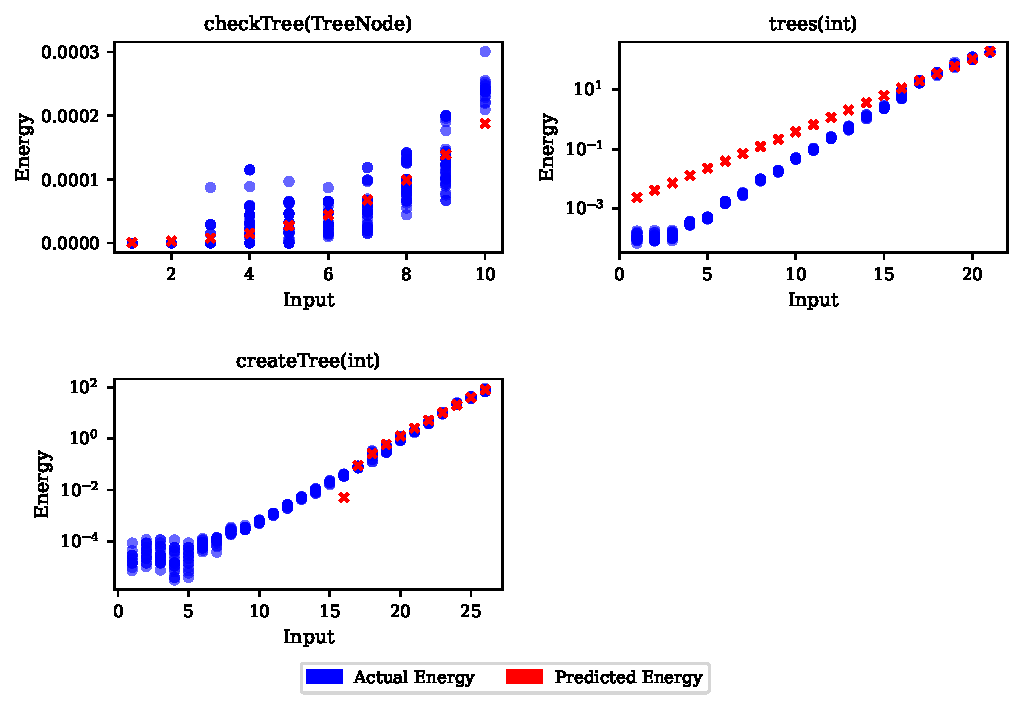
\includegraphics[width=\textwidth]{figures/binarytrees_energy_panel_plot.pdf}
  \caption{Energy for \texttt{BinaryTrees} methods}
  \label{fig:binarytrees_energy_panel_plot}
\end{figure}

\begin{comment}
  
\begin{figure}[htbp]
  \centering
  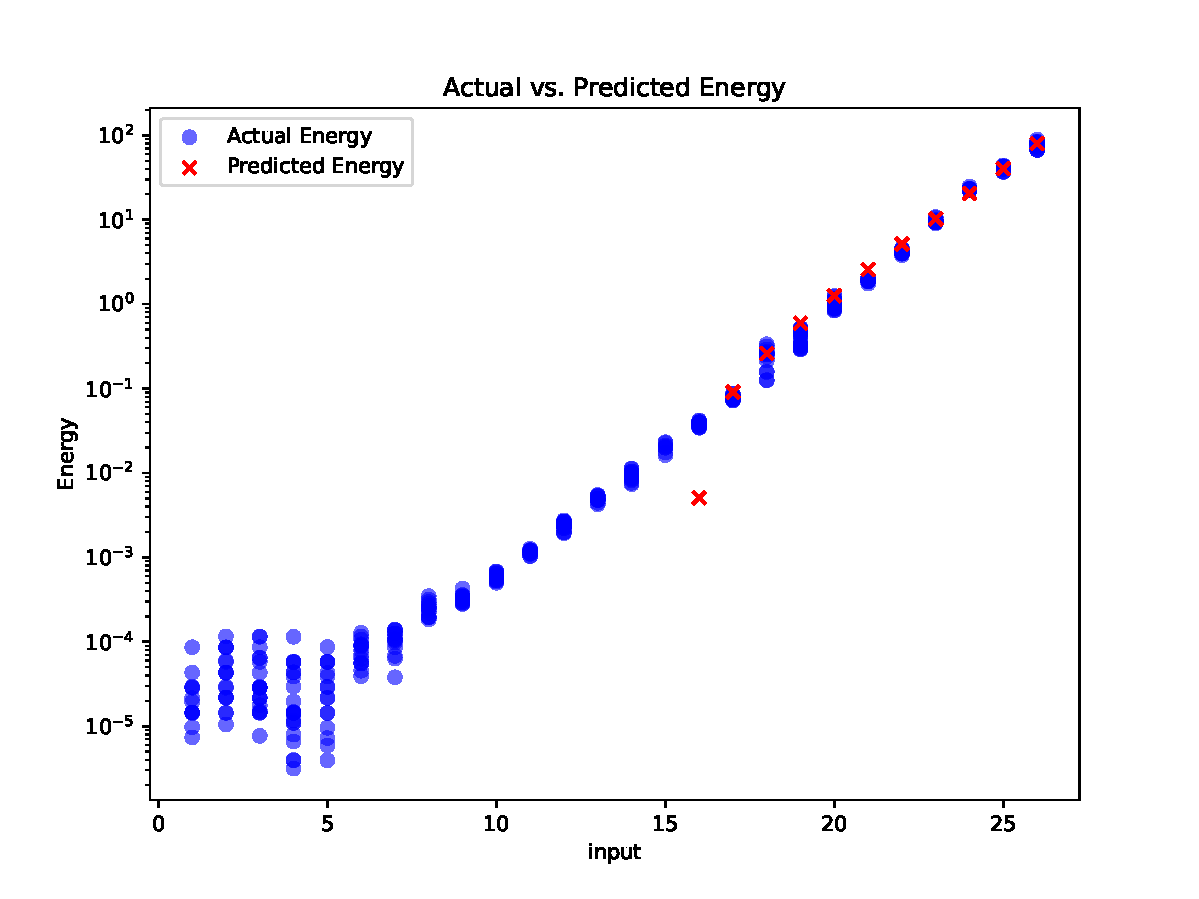
\includegraphics[width = .7 \textwidth]{figures/createTree_plot.pdf}
  \caption{Energy for method \texttt{createTree}}
  \label{fig:createTree_plot}
\end{figure}

\begin{figure}[htbp]
  \centering
  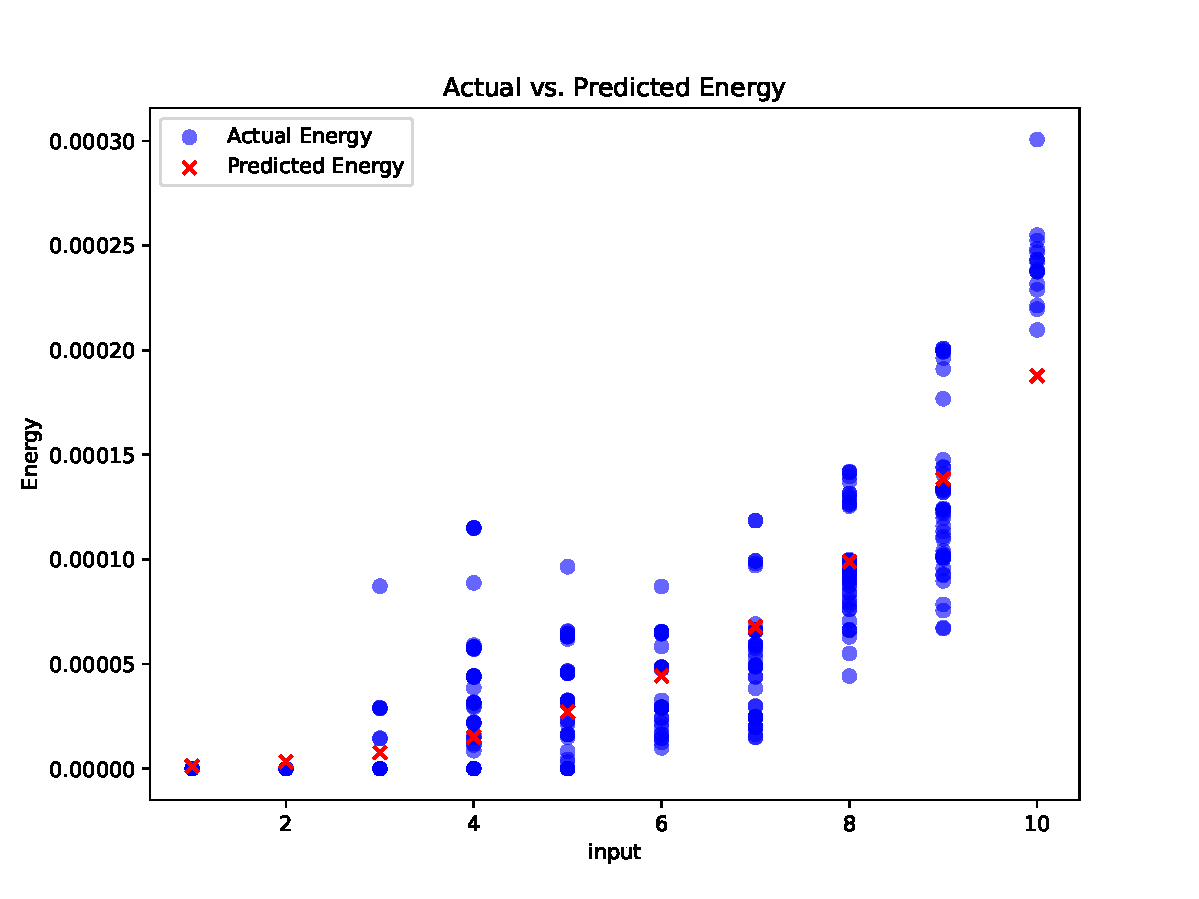
\includegraphics[width = .7 \textwidth]{figures/checkTree_plot.pdf}
  \caption{Energy for method \texttt{checkTree}}
  \label{fig:checkTree_plot}
\end{figure}

\begin{figure}[htbp]
  \centering
  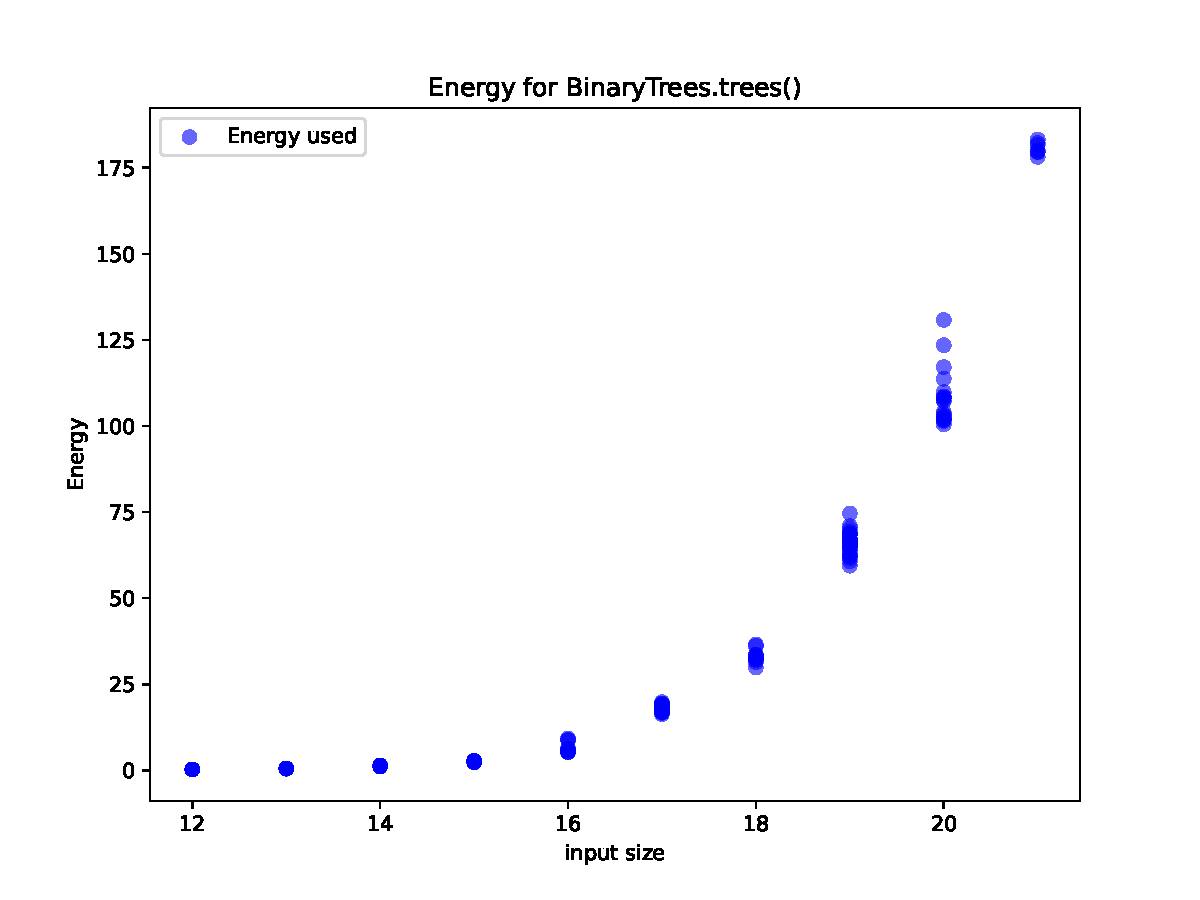
\includegraphics[width = .7 \textwidth]{figures/trees_plot.pdf}
  \caption{Energy for method \texttt{trees}}
  \label{fig:trees_plot}
\end{figure}
\end{comment}

\begin{comment}
  \begin{table}[htbp]
  \centering
  \footnotesize
  \setlength{\tabcolsep}{10pt} % increase column separation
  \makebox[\textwidth][c]{%
    \begin{tabular}{@{}p{5.3cm}@{\hspace{2.5em}}c@{\hspace{1em}}c@{\hspace{1em}}c@{\hspace{1em}}c@{}}
      \toprule
      Method & Input Value & Predicted Energy (J) & Actual Energy Range (J) & Prediction Error (\%) \\
      \toprule

      \multirow{3}{*}{\texttt{BinaryTrees.createTree(int)}}
        & 5 & -0.082 & 1.27e-5 -- 1.49e-5 & 598070 \\
        & 10 & -0.083 & 3.75e-4 -- 4.60e-4 & 19980 \\
        & 23 & 10.26 & 11.78 -- 12.63 & 15.9 \\
        & 26 & 79.90 & 77.29 -- 80.63 & 1.2 \\
      \midrule

      \multirow{3}{*}{\texttt{BinaryTrees.checkTree(TreeNode)}}
        & 5 & 2.71e-05 & 2.63e-6 -- 2.70e-6 & 916 \\
        & 10 & 1.88e-4 & 1.64e-4 -- 1.75e-4 & 10.9 \\
        & 23 & 2.19e-3 & 1.37 -- 1.56 & 99.85 \\
        & 26 & 3.15e-3 & 11.72 -- 13.29 & 99.97 \\
      \midrule

      \multirow{3}{*}{\texttt{BinaryTrees.trees(int)}}
        & 5 & -9.94 & 2.68e-4 -- 3.55e-4 & 1265924 \\
        & 10 & -3.42 & 0.041 -- 0.045 & 8053 \\
        & 23 & 517.89 & 713 -- 800 & 31.59 \\
        & 26 & 2429 & 6260 -- 7111 & 63.66 \\
      \midrule

      \multirow{3}{*}{\shortstack[l]{\texttt{BinaryTrees.checkTree(TreeNode)} +\\\texttt{createTree(int)} +\\\texttt{trees(int)}}}
        & 5 & -4.03 & 2.77e-4 -- 3.44e-4 & 1296569 \\
        & 10 & -3.49 & 4.59e-2 -- 4.77e-2 & 7578 \\
        & 23 & 528.15 & 796 -- 806 & 34.08 \\
        & 26 & 2509 & 7062 -- 7350 & 65.18 \\
      \bottomrule
    \end{tabular}%
  }
  \caption{Comparison of actual and predicted energy consumption for BinaryTrees program}
  \label{tab:energy_comparison_bin_trees}
\end{table}
\end{comment}




%\begin{table}[htbp]
%  \centering
%  \footnotesize
%  \setlength{\tabcolsep}{10pt}
%  \makebox[\textwidth][c]{%
%    \begin{tabular}{@{}p{5.3cm}@{\hspace{2em}}c@{\hspace{1em}}c@{\hspace{1em}}c@{\hspace{1em}}c@{}}
%      \toprule
%      Method & Input Value (\%) & Predicted Energy Simple Model (J) & Predicted Energy Best Model (J) & Actual Energy Range (J) & Prediction Error Simple Model (\%) & Prediction Error Best Model (\%) \\
%      \toprule
%
%      \multirow{3}{=}{\texttt{BinaryTrees.createTree(int)}} 
%        & 10 & -0.083 & 5.63e-04 & 3.75e-4 -- 4.60e-4 & 19980 & 34.97 \\
%        & 23 & 10.26 & 9.42 & 11.78 -- 12.63 & 15.9 & 22.83 \\
%        & 26 & 79.90 & 80.11 & 77.29 -- 80.63 & 1.2 & 1.45 \\
%      \midrule
%
%      \multirow{3}{=}{\texttt{BinaryTrees.checkTree(TreeNode)}}
%        & 10 & 1.88e-4 & 2.28e-04 & 1.64e-4 -- 1.75e-4 & 10.9 & 34.4 \\
%        & 23 & 2.19e-3 & 2.43e-03 & 1.37 -- 1.56 & 99.85  & 99.83\\
%        & 26 & 3.15e-3 & 3.53e-03 & 11.72 -- 13.29 & 99.97 & 99.97\\
%      \midrule
%
%      \multirow{3}{=}{\texttt{BinaryTrees.trees(int)}}
%        & 10 & -3.42 & 1.69 & 0.041 -- 0.045 & 8053 & 3833 \\
%        & 23 & 517.89 & 798 & 713 -- 800 & 31.59 & 5.49\\
%        & 26 & 2429 & 39754 & 6260 -- 7111 & 63.66 & 494.63 \\
%      \midrule
%
%      \multirow{3}{=}{\parbox{5.3cm}{\centering\texttt{BinaryTrees.checkTree(TreeNode) +\\ createTree(int) + trees(int)}}}
%        & 10 & -3.49 & 4.59e-2 -- 4.77e-2 & 7578 \\
%        & 23 & 528.15 & 796 -- 806 & 34.08 \\
%        & 26 & 2509 & 7062 -- 7350 & 65.18 \\
%      \bottomrule
%    \end{tabular}%
%  }
%  \caption{Comparison of actual and predicted energy consumption for BinaryTrees program}
%  \label{tab:energy_comparison_bin_trees}
%\end{table}

Table~\ref{tab:energy_comparison_bin_trees} presents the detailed information about the energy consumption of the BinaryTrees program\wo{de novo os resultados parecem super estimados. Tens uma intuição sobre isso?}. It is noticeable that the values predicted are not the most accurate, for some inputs it has good accuracy, for example, the method \texttt{createTree} has good accuracy for the input \texttt{26}. For other methods, such as \texttt{trees} it does not. Again as the previous experiment, the tool is not very accurate in terms of absolute values, and in this case for methods that change their energy considerably with minimum increase in the input, the models have a harder time to predict. The tool demonstrates good relative energy prediction, as input values increase, the predicted energy consumption also increases, and it decreases correspondingly when the inputs are reduced.


\begin{table}[htbp]
  \centering
  \footnotesize
  \setlength{\tabcolsep}{10pt} % increase column separation
  \makebox[\textwidth][c]{%
    \begin{tabular}{@{}p{5.3cm}@{\hspace{2.5em}}c@{\hspace{1em}}c@{\hspace{1em}}c@{\hspace{1em}}c@{}}
      \toprule
      Method & Input Value & Predicted Energy (J) & Actual Energy Range (J) & Prediction Error (\%) \\
      \toprule

      \multirow{3}{*}{\texttt{BinaryTrees.createTree(int)}}
        & 5 & -0.082 & [1.27e-5, 1.49e-5] & 598070 \\
        & 10 & -0.083 & [3.75e-4, 4.60e-4] & 19980 \\
        & 23 & 10.26 & [11.78, 12.63] & 15.9 \\
        & 26 & 79.84 & [77.29, 80.63] & 1.12 \\
      \midrule

      \multirow{3}{*}{\texttt{BinaryTrees.checkTree(TreeNode)}}
        & 5 & 2.71e-05 & [2.63e-6, 2.70e-6] & 916 \\
        & 10 & 1.88e-4 & [1.64e-4, 1.75e-4] & 10.9 \\
        & 23 & 2.19e-3 & [1.37, 1.56] & 99.85 \\
        & 26 & 3.15e-3 & [11.72, 13.29] & 99.97 \\
      \midrule

      \multirow{3}{*}{\texttt{BinaryTrees.trees(int)}}
        & 5 & 0.02 & [2.68e-4, 3.55e-4] & 7202 \\
        & 10 & 0.38 & [0.041, 0.045] & 786 \\
        & 23 & 581 & [713, 800] & 23.23 \\
        & 26 & 3152 & [6260, 7111] & 52.86 \\
      \midrule

      \multirow{3}{*}{\shortstack[l]{\texttt{BinaryTrees.checkTree(TreeNode)} +\\\texttt{createTree(int)} +\\\texttt{trees(int)}}}
        & 5 & -0.06 & [2.77e-4, 3.44e-4] & 19341 \\
        & 10 & 0.30 & [4.59e-2, 4.77e-2] & 541 \\
        & 23 & 591 & [796, 806] & 26.20 \\
        & 26 & 3232 & [7062, 7350] & 55 \\
      \bottomrule
    \end{tabular}%
  }
  \caption{Comparison of actual and predicted energy consumption for BinaryTrees program}
  \label{tab:energy_comparison_bin_trees}
\end{table}

\wo{acho que podes juntar as tabelas 5.4, 5.5 e 5.6 em uma só. Pq só falas dos métodos de BinaryTrees, e não dos outros? As figuras falam nomes de métodos sem dizer de onde vem. Os benchmarks não tem metodos? Eu não gosto muito de todas essas tabelas e plots separados. Vê se consegues juntar mais.}


The Figure~\ref{fig:benchmark_energy_panel_plot}, shows the measured energy with the predictions, and it is observable that the energy grows quickly as the input also increases. Both the Table~\ref{tab:energy_comparison_benchmark} and the Figure~\ref{fig:benchmark_energy_panel_plot}, confirm that for inputs lower than ten, the model has difficulties predicting.


{\color{blue}For the \texttt{spectralnorm} benchmark, several methods are involved: \texttt{Approximate(int)}, \texttt{A(int, int)}, \texttt{MultiplyAv(int, \allowbreak\ double[],\allowbreak\ double[])}, \texttt{MultiplyAtv(int,\allowbreak\ double[],\allowbreak\ double[])}, and \texttt{MultiplyAtAv(int,\allowbreak\ double[],\allowbreak\ double[])}. While all these methods were included during the training, the analysis focused on \texttt{Approximate(int)}. This is because it is the method invoked by the \texttt{main} function and is responsible for the core computation of the program.}
The model obtained for the \texttt{spectralnorm} case prove quite effective discovering the pattern of the energy usage of the method, being the input the main feature that help achieve it, as Figure~\ref{fig:benchmark_energy_panel_plot} shows, the prediction and measured values are almost similiar, and the prediction follows the curve of the mesaured energy. The concrete values can be seen in the Table~\ref{tab:energy_comparison_benchmark}, and it illustrates that the higher inputs tend to have higher accuracy as well.


{\color{blue}For the \texttt{spectralnorm} benchmark, several methods are involved: \texttt{offsetMomentum(\allowbreak\ double,\allowbreak\ double,\allowbreak\ double)},
\texttt{energy()}, \texttt{advance(double)}. The methods included in the training were \texttt{energy()}, \texttt{advance(double)}. However, the \texttt{energy()} method did not receive any inputs and lacked features that the model could use to differentiate energy consumption across executions. As a result, the model learned to predict a constant value for this method. Consequently, only \texttt{advance(double)} was selected for detailed analysis in this benchmark experiment.}
This time the resulting model had difficulties predicting the energy for the given method, as shown in the Table~\ref{tab:energy_comparison_benchmark}. The Figure~\ref{fig:benchmark_energy_panel_plot} also shows an interesting behavior of the measured energy, which might explain why the model accuracy is so low.


\begin{table}[htbp]
  \centering
  \footnotesize
  \setlength{\tabcolsep}{10pt} 
  \makebox[\textwidth][c]{%
    \begin{tabular}{@{}p{5.3cm}@{\hspace{2.5em}}c@{\hspace{1em}}c@{\hspace{1em}}c@{\hspace{1em}}c@{}}
      \toprule
      Method & Input Value & Predicted Energy (J) & Actual Energy Range (J) & Prediction Error (\%) \\
      \toprule

      \multirow{3}{*}{\texttt{NBodySystem.advance(double)}}
        & 100 & 4.4e-5 & [3.02e-6, 3.25e-6] & 1302 \\
        & 1000 & 4.85e-5 & [2.93e-6, 3.20e-6] & 1480 \\
        & 10,000 & 4.11e-5 & [2.97e-6, 3.15e-6] & 1243 \\
        & 100,000 & 5e-5 & [2.97e-6, 3.15e-6] & 1533 \\
      \midrule
      \multirow{3}{*}{\texttt{fannkuch(int)}}
        & 5 & 3.68e-3 & [8.04e-5, 9.51e-5] & 4089 \\
        & 10 & 8.69 & [3.72, 8.52] & 42 \\
        & 11 & 105.26 & [87.25, 111.36] & 6 \\
        & 12 & 1275 & [1187, 1585] & 8 \\
      \midrule
      \multirow{3}{*}{\texttt{spectralnorm().Approximate(int)}}
        & 10 & 6.29e-3 & [2.65e-4, 2.85e-4] & 2187 \\
        & 100 & .08 & [0.02, 0.021] & 297 \\
        & 1000 & 2.67 & [2.0, 2.22] & 26 \\
        & 10,000 & 212 & [205, 207] & 2.9 \\
      \bottomrule
    \end{tabular}%
  }
  \caption{Comparison of actual and predicted energy consumption for nBody, fannkuch and spectralnorm program}
  \label{tab:energy_comparison_benchmark}
\end{table}


\begin{comment}
  \begin{table}[htbp]
  \centering
  \footnotesize
  \setlength{\tabcolsep}{10pt}
  \makebox[\textwidth][c]{%
    \begin{tabular}{@{}p{5.3cm}@{\hspace{2.5em}}c@{\hspace{1em}}c@{\hspace{1em}}c@{\hspace{1em}}c@{}}
      \toprule
      Method & Input Value & Predicted Energy (J) & Actual Energy Range (J) & Prediction Error (\%) \\
      \toprule

      \multirow{3}{*}{\texttt{fannkuch(int)}}
        & 5 & 3.68e-3 & [8.04e-5, 9.51e-5] & 4089 \\
        & 10 & 8.69 & [3.72, 8.52] & 42 \\
        & 11 & 105.26 & [87.25, 111.36] & 6 \\
        & 12 & 1275 & [1187, 1585] & 8 \\
      \bottomrule
    \end{tabular}%
  }
  \caption{Comparison of actual and predicted energy consumption for fannkuch redux program}
  \label{tab:energy_comparison_fannkuch_redux}
\end{table}

\begin{table}[htbp]
  \centering
  \footnotesize
  \setlength{\tabcolsep}{10pt}
  \makebox[\textwidth][c]{%
    \begin{tabular}{@{}p{5.3cm}@{\hspace{2.5em}}c@{\hspace{1em}}c@{\hspace{1em}}c@{\hspace{1em}}c@{}}
      \toprule
      Method & Input Value & Predicted Energy (J) & Actual Energy Range (J) & Prediction Error (\%) \\
      \toprule

      \multirow{3}{*}{\texttt{spectralnorm().Approximate(int)}}
        & 10 & 6.29e-3 & [2.65e-4, 2.85e-4] & 2187 \\
        & 100 & .08 & [0.02, 0.021] & 297 \\
        & 1000 & 2.67 & [2.0, 2.22] & 26 \\
        & 10,000 & 212 & [205, 207] & 2.9 \\
      \bottomrule
    \end{tabular}%
  }
  \caption{Comparison of actual and predicted energy consumption for spectral-norm program}
  \label{tab:energy_comparison_spectral_norm}
\end{table}
\end{comment}



\begin{figure}[htbp]
  \centering
  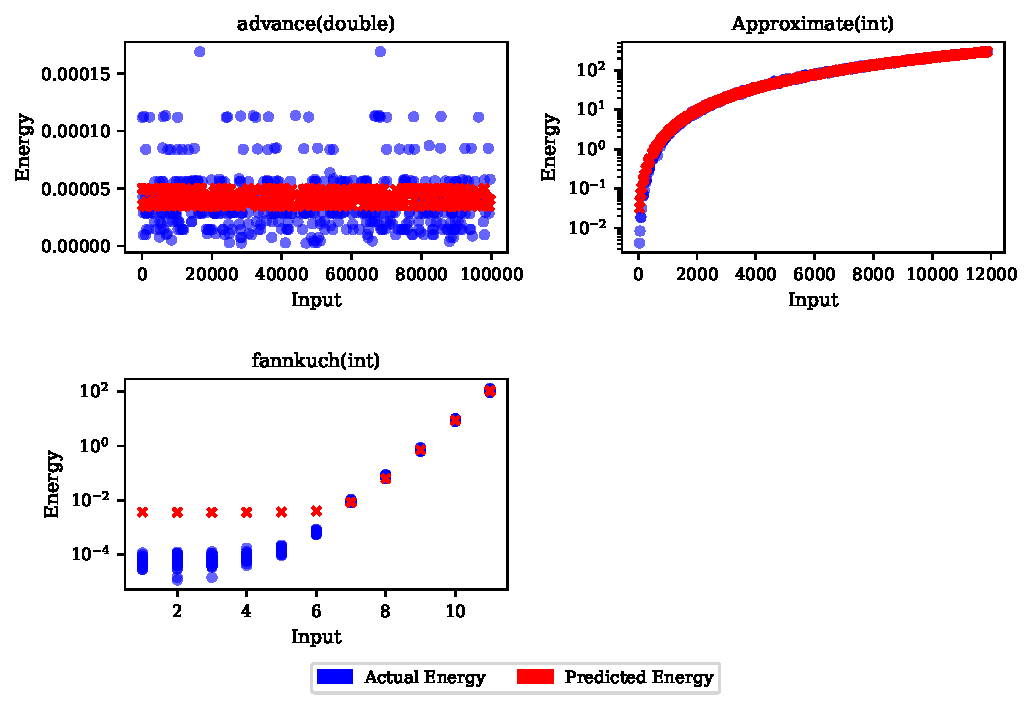
\includegraphics[width=\textwidth]{figures/benchmark_energy_panel_plot.pdf}
  \caption{Energy for \texttt{advance}, \texttt{Approximate} and \texttt{fannkuch} methods}
  \label{fig:benchmark_energy_panel_plot}
\end{figure}



\begin{comment}
  

\begin{figure}[htbp]
  \centering
  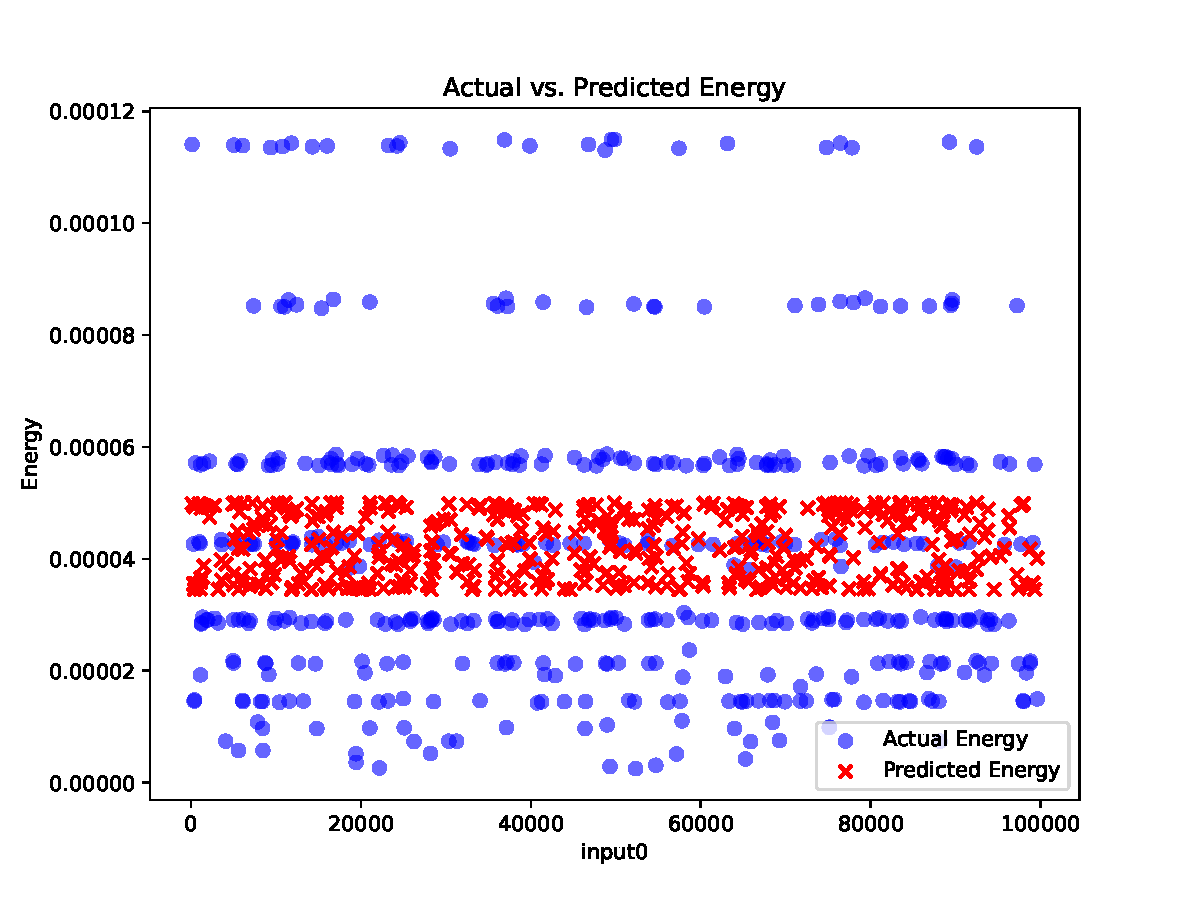
\includegraphics[width = .7 \textwidth]{figures/advance_plot.pdf}
  \caption{Energy for method \texttt{advance}}
  \label{fig:advance_plot}
\end{figure}

\begin{figure}[htbp]
  \centering
  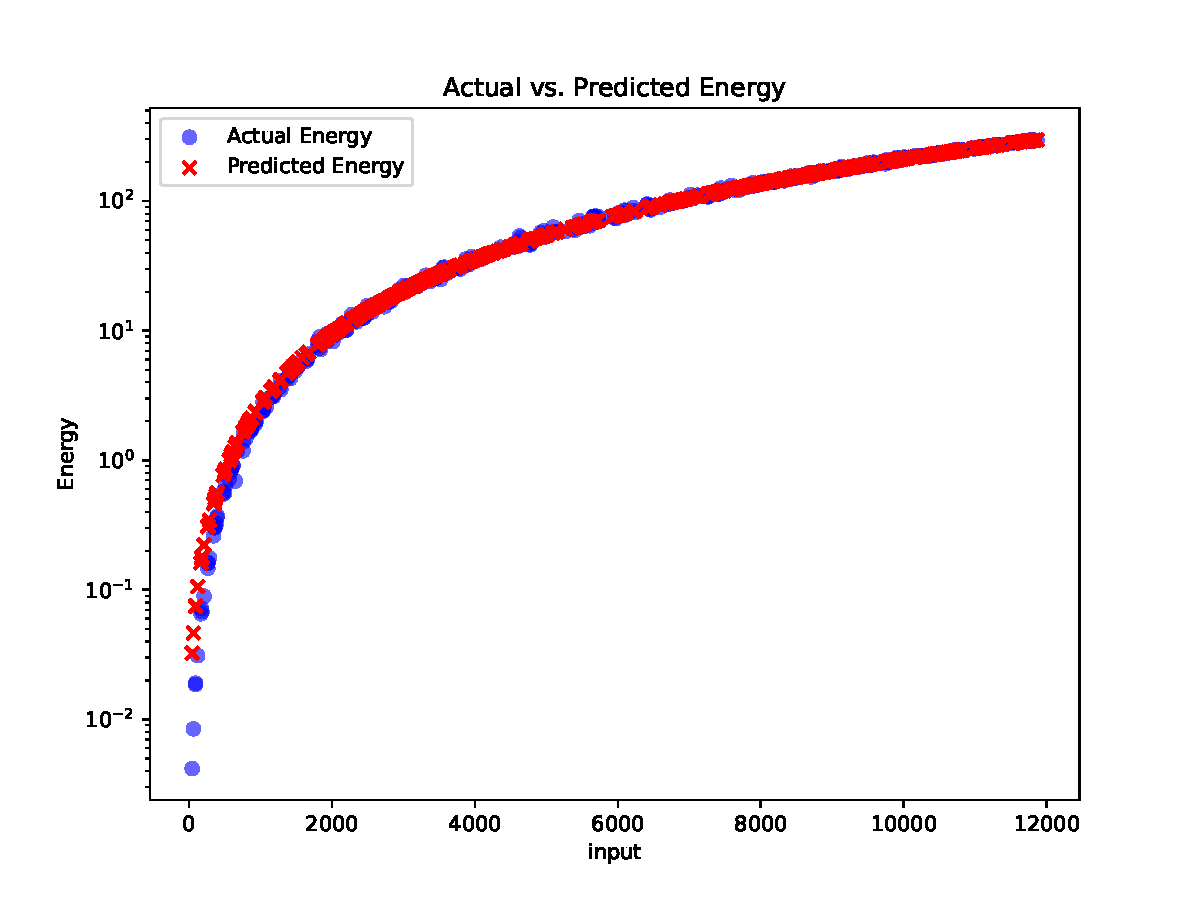
\includegraphics[width = .7 \textwidth]{figures/approximate_plot.pdf}
  \caption{Energy for method \texttt{approximate}}
  \label{fig:approximate_plot}
\end{figure}

\begin{figure}[htbp]
  \centering
  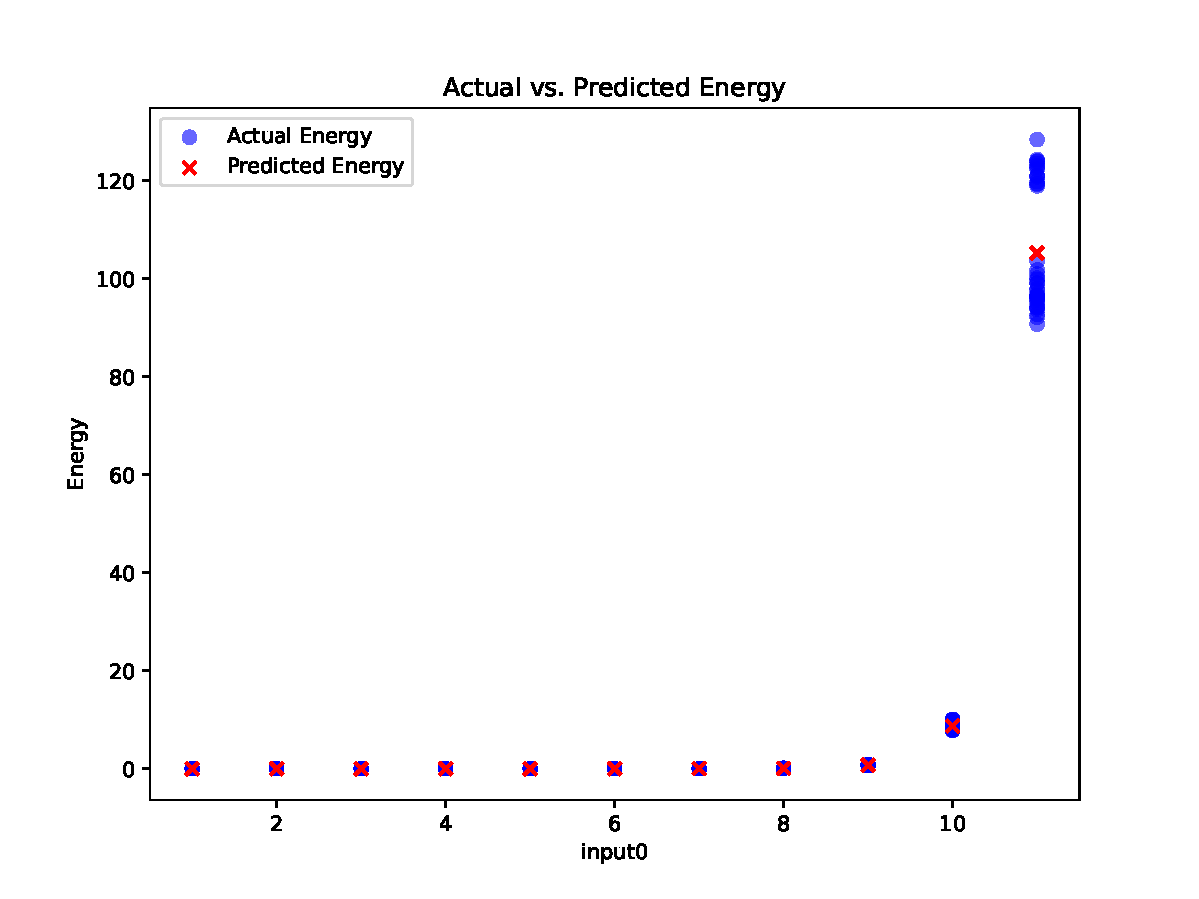
\includegraphics[width = .7 \textwidth]{figures/fannkuch_plot.pdf}
  \caption{Energy for method \texttt{fannkuch}}
  \label{fig:fannkuch_plot}
\end{figure}
\end{comment}


To achieve better results it could be possible to improve the feature's selection by incorporating characteristics that better capture the program complexity and increase the maximum input available for each program generated in order to better represent the high-energy regions of execution.


This experiment also tests how pratical it is to actually measure a custom program. 
The \texttt{BinaryTrees} program, from how it is implemented on the website it needs some small adjustments in order to work with our framework. First, the program does not have a constructor for the class \texttt{TreeNode} which does not allow the program generator to populate the programs correctly, as the program on the website uses a custom method that create the nodes. Without this change, the methods that required \texttt{TreeNode} as input would be simply receiving an empty Object, as the constructor was also empty, making their generation useless as every program would be the same.
With that said, the only adjustments made to the class were, a new private empty constructor, that can only be accessed inside the class, so the generator does not detect it and use it, as the generator always tries to use the smallest one available, so it is important that the empty constructor is private. And it was added a new constructor, this one public, that had the same logic as the method that created the nodes. Now the methods that use \texttt{TreeNode} can be generated as the constructor can call the public constructor that has the similar behavior of the \texttt{createTree(int)} method. These changes do not impact how the program, or methods behave and only helps the program generation.
Aside from the \texttt{BinaryTrees} program, the others were even less troubled, as the \texttt{fannkuch-redux} and \texttt{spectral-norm} required no changes, apart from the package declaration, and the \texttt{n-body} program only required to divide the internal classes into more Java classes resulting in three files — \texttt{n-body.java}, \texttt{NBodySystem.java}, and \texttt{Body.java}.


This experiment objective's was not focused only on achieving the highest accuracy possible. It was also made to prove that it is possible to use the framework to test more interesting and complex cases. And it was proven that with minimal changes, it was possible to mass generate programs, collect data and train models, for four different programs. While it may not work universally for all programs, since creating a framework general enough to handle every case is challenging, this experiment demonstrates that analyzing custom programs is possible.


\section{Analysis} \label{sec:analysis}

In this chapter the results obtain for the custom programs will be analyzed.

In most of the experiments, it was observed that the energy consumption curve followed the input values, meaning the model's predicted energy usage was largely dependent on the input. Since the tested programs involved computationally intensive tasks, increasing the input also led to longer execution times, which in turn caused higher energy consumption, indicating a strong correlation between execution time and energy usage. 
For the methods where a lower input was enough to generate a benchmark that would run for an acceptable amount of time, the models could predict better, as a small increase in the input would affect the energy consumption by a significant amount. However, to prioritize accurate predictions for higher input values, many models tended to fail in predicting energy usage for the lower input range.

As it is now, the most important feature collected from the benchmarks is the input, and it showed to be effective in helping the models outputting a reliable prediction model. However, it is possible to see that it is the only variable that can help the models predict in this case. They could benefit from a more diverse set of features that could include dynamic features, for instance, time of execution, processor cycles or other low-level metrics. Using more features could help the overall accuracy of the models.

From the experiments conducted, the one that displayed the most unusual result, was the \texttt{advance} method from the \texttt{nbody} program. The concrete reason to why the predictions and the measured values are not as accurate as the those of other methods, is not known for sure, however, there is a hypothesis. The methods \texttt{advance} required higher inputs. Since the input generator is limited to a maximum threshold, the benchmarks generated were also capped to that value. This would make that an input of 1 or 100,000 would spend in general the same amount of energy, making the input a bad decision factor for the model. Increasing the input could lead to a better model for this particular method, but could also increase the search time of the maximum inputs in the generator.

Overall, the results indicate that while the models are capable of producing reliable energy consumption predictions under certain conditions, their accuracy and adaptability could be significantly improved with a richer and more diverse feature set.



%\wo{Escreve aqui uma secção de análise, onde tu analisas os resultados que obtiveste. O que é que tu achas que correu bem? O que é que correu mal? Pq o resultados do Nbody são tão ruins? pq o fannkuch é incrivelmente bom? Pq a maioria deles consegue prever melhor quando temos um input maior? Essa é parte que vai mostrar que tu percebeu o que se passou no teu trabalho.}






\section{Limitations and Challenges} \label{sec:limitations_and_challenges}

During program generation, most of the tested collections focused on \texttt{List}, \texttt{Set}, and \texttt{Map}. However, programs were also generated for another collection category, the \texttt{Math} library. This introduced an issue. The computations in these programs were extremely fast, completing too quickly for PowerJoular to measure any meaningful energy consumption. As a result, all energy readings for the \texttt{Math} programs were reported as 0J.
We were able to identify that the source of the problem was the array sizes used to hold the method parameters. While the three predefined array sizes worked well for \texttt{List}, \texttt{Set}, and \texttt{Map}, they were too small for the \texttt{Math} library. The smaller input sizes caused the Math computations to execute very fast, not giving PowerJoular enough time to capture energy usage.
This highlights a challenge in energy profiling: some collections, especially those involving lightweight or highly optimized operations like Math functions, may be difficult to measure accurately. One possible solution would be to determine array sizes during program generation, large enough to ensure that each program runs for at least one second, giving PowerJoular sufficient time to measure energy consumption. However, implementing this would significantly increase the time required for program generation, as it would involve exploring many more combinations of input sizes to find suitable configurations. \wo{A gente já não faz isso?}

Another important factor is that the tool is not able to predict energy when threads are involved, as the programs generated only used a single thread, subsequently the models will not have that factor into account. This limitation exists because measuring and modeling the energy usage of multithreaded programs is particularly challenging due to factors like concurrent execution, thread scheduling, and synchronization overhead. However, threading can deeply impact the energy usage of a program, as a program execution stop being strictly linear, and can have multiple simultaneous computations, potentially increasing the code energy consumption.


A limitation detected during the experimentation of analyzing an external program, was how the inputs on some programs are defined. For example, a program can have a method that receives a \texttt{String}, however, when inside the method it decides to convert the \texttt{String} to \texttt{int} and use it as an \texttt{Integer}, making it so a method that actually uses \texttt{Integers} and not \texttt{Strings}. Although it is easily noticeable by human eye, the program generator cannot understand this kind of context changes as easy, and it would start generating inputs for \texttt{Strings} instead of \texttt{Integers}, which would fail in the program generation. A good example of this usage is when the main function is called and receives the arguments in the \texttt{String[]} and then it uses its values in different variables.





%In the start of the project, some tools were tested in order to see how to get the energy profiles for later use. The tools tested were PowerJoular, Powertop, Perf and JoularJx.
%
%Perf is a Linux tool primarily designed for analyzing application performance characteristics rather than precise energy measurement. While it can provide some energy-related metrics, its measurements tend to be imprecise. In this context, Perf was used mainly to get a rough idea of energy consumption and to serve as an alternative when more accurate tools were unavailable.
%
%Powertop was also tested, but it could only perform energy measurements on laptops, as it relies on battery drain data to calculate energy consumption. Since this approach doesn't align with our specific requirements, we considered Powertop as a last-resort option.
%
%JoularJx is an energy measurement tool capable of measuring the consumption of Java programs and its methods. However, it is not as precise as other tools as it requires to measure the entire start of the JVM and whole functions instead of small code blocks.
%
%As described in the \ref{sec:background_energy}, PowerJoular is the best option. As a command line program it can be easily adapted to measure any program or code snippet in most languages. So it was combined with the framework experiment-runner, that facilitates the process.
%
%Initially, JoularJx and the experiment-runner using PowerJoular were used to explore their capabilities and familiarize with the tools. A sample Fibonacci program written in Java and C was used as a test case. However, the energy measurements provided by the two tools differed, and the experiment runner occasionally encountered errors. Later, it was determined that these problems were due to incorrect use of the framework. However, it was still decided the best approach was to make a new orchestrator similar to the Experiment-Runner, but simpler and specifically focused on measuring process energy consumption using PowerJoular. A Java-based orchestrator was initially developed because the Fibonacci implementation was also in Java. However, when tested, the energy measurement results differed significantly from those of the experiment runner, even though the main difference was the programming language (Java vs. Python).
%
%To further analyze these inconsistencies, another orchestrator was developed in Python. This allowed for a closer examination of the differences in energy measurements and a deeper understanding of the behavior of the tools.
%
%Using the process explained on \ref{chapter:approach} it was noticeable that the Java orchestrator was getting significantly more energy consumption than the Python one, which is not very logical, since they both target the same program. So, to try and check which one was having problems, two more orchestrators were implemented, one in C and another in bash.
%
%After running the tests again it was possible to see that the Python orchestrator was getting values way more different from the other three orchestrators as show in Figure \ref{fig:4_orchs_comparison}.
%The figure contains 100 runs of the Fibonacci recursive program written in Java and order by the less energy to the highest energy. And it shows the energy reads for the four different orchestrators used. The labels contain the average energy values and its standard deviation.
%
%Further analysis of the orchestrators revealed a notable difference in behavior. When the Python orchestrator was running, both the parent and child processes consumed CPU resources. In contrast, the other orchestrators (Java, C, and Bash) showed CPU usage only in the child process. This disparity may explain why PowerJoular reported lower energy consumption for the Python orchestrator. Since the CPU load was shared between the parent and child processes, PowerJoular, which measures energy only for the child process (the target Fibonacci program), captured less total energy usage.
%Since the experiment runner included an example demonstrating how to use the framework with PowerJoular, the authors were made aware of this potential conflict when launching PowerJoular from Python.
%
%\begin{figure}%[h]
%  \centering
%  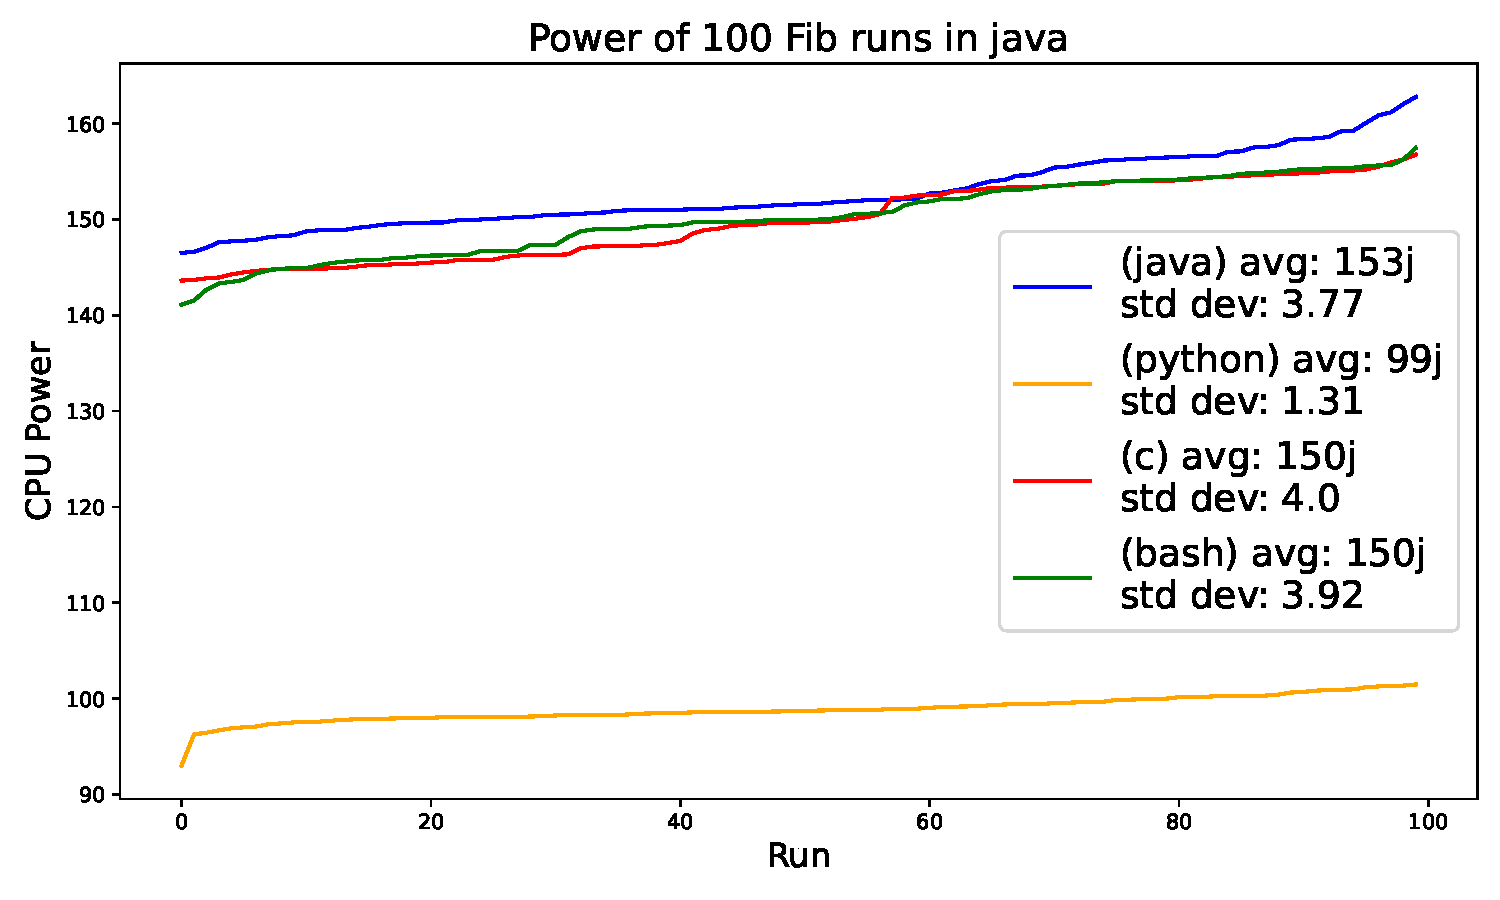
\includegraphics[width = 0.5 \textwidth]{figures/4_orchestrators_comparison.pdf}
%  \caption{orchestrators comparison}
%  \label{fig:4_orchs_comparison}
%\end{figure}